\documentclass[10pt]{beamer}

\usetheme{Montpellier}
\usecolortheme{whale}

\usepackage[T1]{fontenc}
\usepackage{lmodern}

\usepackage{mathtools}
\usepackage[binary-units]{siunitx}
\usepackage{amsmath}
\usepackage{listings}
\usepackage{mdframed}
\usepackage{minted}
\usepackage{xcolor}

\usepackage{parskip}
\usepackage{substr}
\usepackage{hyperref}
\usepackage{etoolbox}
\usepackage{tipa}
\usepackage{cprotect}
\usepackage{booktabs}
\usepackage{silence}
\usepackage[backend=biber, style=ieee]{biblatex}
\usepackage[english,ngerman]{babel}
\usepackage{csquotes}

\definecolor{lg}{gray}{0.95}
\hypersetup{colorlinks = true, urlcolor=blue, linkcolor=white}
\WarningFilter{biblatex}{Patching footnotes failed}

\renewcommand*{\bibfont}{\tiny}

\bibliography{resources.bib}

\title{\textbf{Operating Systems}}
\subtitle{Tutorial 2}
\author{Fabian Klopfer}
\date{\today}

\begin{document}
\frame{\titlepage}


\begin{frame}{Intro}
\begin{itemize}
 \item Pingo Polls
 \item Has everybody managed to see the annotations in the correction?
\end{itemize}
\end{frame}

\begin{frame}[allowframebreaks]{Exercise sheet 1}
\begin{itemize}
 \item \textbf{If you take initialization into account}, the  exact answer for exercise 4.1 is $1 \cdot 10^9 -2$ Op \\
 \begin{itemize}
  \item Why -2? Before the first instruction can be executed you need to fetch one (1ns) and decode one (1ns). 
  \item Why not -5? Theoretically it suffices if one pipeline level is ready. One does not need to wait for all pipelines to fetch and decode.
  \item Practically this is of course not the case: For example if branches are predicted incorrectly the whole pipeline is flushed. Also on arrival of an interrupt and after it's handling the pipeline is flushed. Faults and traps make the CPU push the pipeline to the stack $\rightarrow$ you also lose some cycles for pushing \& reloading the pipeline.
 \end{itemize}
 \item actually asked for was the \textbf{throughput}! This is $1 \cdot 10^9$ Op/s\\ no matter the initial latency!
 
 \framebreak
\item \textbf{ALWAYS} check your code with following flags. Notice that thread can not be used with address and undefined. More information is available \href{https://gcc.gnu.org/onlinedocs/gcc/Instrumentation-Options.html}{here}.
\begin{itemize}
 \item Always do one pass with \mintinline{bash}{-fsanitize=address -fsanitize=undefined} to check e.g. array bounds, memory leaks and other issues connected to memory.
 \item For code that shall be thread safe use \mintinline{bash}{-fsanitize=thread}.
 \item There are even more utilities that check things at runtime for you, check the  \href{https://gcc.gnu.org/onlinedocs/gcc/Instrumentation-Options.html}{doumentation}.
\end{itemize}

\end{itemize}
\end{frame}

\section{Exercise Sheet 1}
\frame{\sectionpage}
\begin{frame}[allowframebreaks]{Exercise 1}
    	\begin{enumerate}
		\item What is the difference between program code and process? \\
		\alert{Process: Running program; code executing dynamically in a context.}
		
		\item What is a process control block and which information does it contain? \\
		\alert{Data structure containing context of a process
		Used by OS for maintenance and scheduling}
        \begin{figure}
          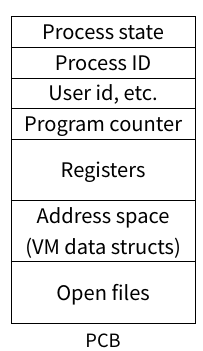
\includegraphics[keepaspectratio, width=0.3\textwidth, height=0.6\textheight-2\baselineskip-2\baselineskip]{img/000_pcb.png}
        \end{figure}
		
		
		\item What is the difference between a mode switch and a process switch? \\
		\alert{A process switch (context switch) stores the state of a process and loads the state of another process. \\
		A mode switch changes switches between user mode and kernel mode, due to an interrupt, trap or exception.}
		
		\item What is the key difference between processes and threads? \\
		\alert{Processes have a full context. \\
		Threads share the context of their process.}
		\framebreak
		
		\item Does each thread have its own stack? \\
		\alert{Each thread has an own stack and register values.}
		        \begin{figure}
          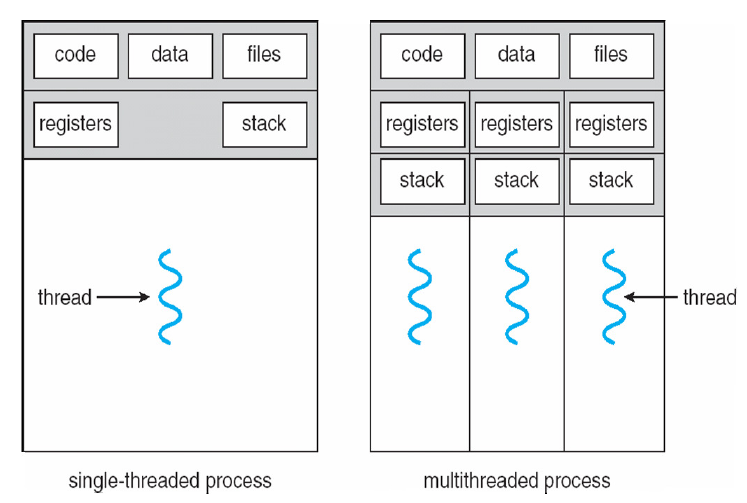
\includegraphics[keepaspectratio, width=0.6\textwidth, height=0.6\textheight-2\baselineskip-2\baselineskip]{img/000_proc_threads.png} \\
        \end{figure}
		\framebreak
		
		\item The management of threads by an operating system can happen in kernel space or in user space. Name an advantage and a disadvantage of user threads compared to kernel threads. \\
		\alert{
		\begin{itemize}
		 \item[+] No mode switch for a thread switch, platform independent
		 \item[-] Error prone, if a thread blocks the whole process does
		\end{itemize}
		}
        \begin{figure}
          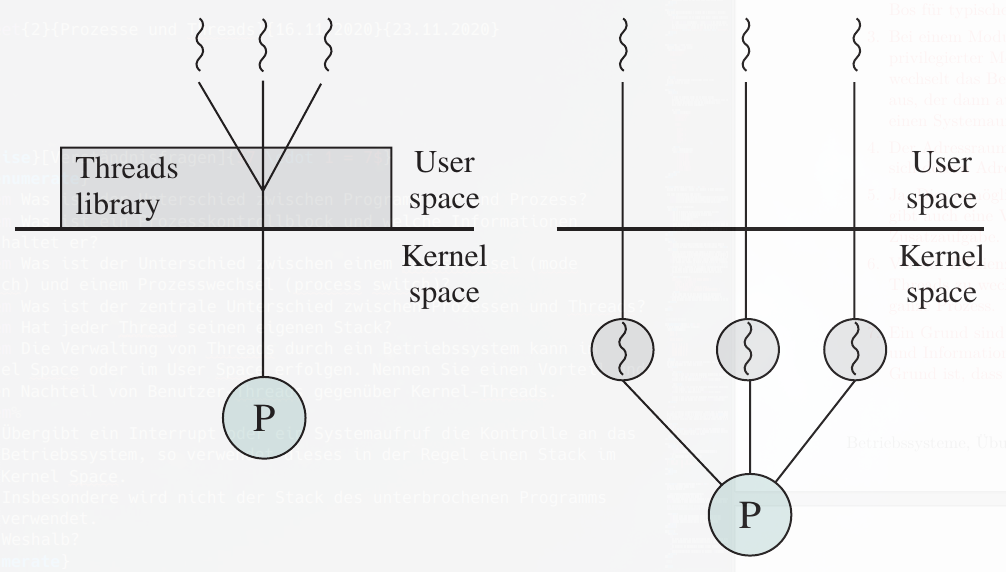
\includegraphics[keepaspectratio, width=0.6\textwidth, height=0.6\textheight-2\baselineskip-2\baselineskip]{img/000_user_threads.png} \\
        \end{figure}
    \framebreak
		
		\item%
			If an interrupt or a system call passes control to the operating system, the latter usually uses a stack in kernel space.
            In particular, the stack of the interrupted program is not used. Why?
            \alert{
            \begin{itemize}
             \item Stack might be too small when user program uses a lot
             \item Stack might be read out after returning to the user program \\
                sub esp X
            \end{itemize}
            }

	\end{enumerate}
\end{frame}

\begin{frame}[allowframebreaks]{Exercise 2}
\begin{enumerate}
		\item%
			Five programs are running on a computer system.
			At any given time, each of the programs waits for input/output independently of the others with a probability of $1/2$.
			What is the average fraction of CPU time that is wasted? \\
			\alert{Tanenbaum~\autocite{tanenbaum} p. 96: $Pr(\text{All Processes do IO}) = p^n$
			with $p$ the average probability to do IO and $n$ the number of processes.
			\[\Rightarrow \frac{1}{2}^5 = \frac{1}{32} \]}
        \framebreak
		\item%
			A computer system has a memory of \SI{16}{\gibi\byte}, of which the operating system occupies \SI{768}{\mebi\byte}.
			For simplicity, we assume that all processes use \SI{256}{\mebi\byte} of memory and behave the same way.
			CPU utilization should be \SI{99}{\percent}.
			What is the maximum amount of time (in percent) each process can use for input/output? \\ \vspace{0.5cm}
			\alert{$\frac{16\si{\gibi\byte}}{256\si{\mebi\byte}} = 64$ blocks. \\
			OS uses 3 blocks $\Rightarrow$ 61 blocks used for 61 processes. \\
			Tanenbaum~\autocite{tanenbaum} p. 96: CPU utilization = $1-p^n$ \\
			\[ 0.99 = 1-p^{61} \Leftrightarrow 0.01 = p^{61} \Leftrightarrow p = 0.01^{\frac{1}{61}} = 0.92728 \sim 93\% \]}
	\end{enumerate}
\end{frame}

\begin{frame}[allowframebreaks]{Exercise 3}
		Consider the following \mintinline{bash}{C} program:
	\inputminted{c}{code/fork.c}
	How many \textbf{child} processes are created when the program is executed?
	Describe briefly what happens. \\
    \alert{Pingo poll \& execute it}
\end{frame}

\begin{frame}[allowframebreaks, fragile]{Exercise 4}
	 Define the terms ``synchronous'' and ``asynchronous''
    \alert{
    \begin{itemize}
     \item Synchronous: Coordinated with others (e.g. threads, processes, devices, nodes), e.g. actively wait for completion of previous step
     \item Asynchronous: The timing is detached from others and signalled instead 
    \end{itemize}
    }
    \begin{figure}
          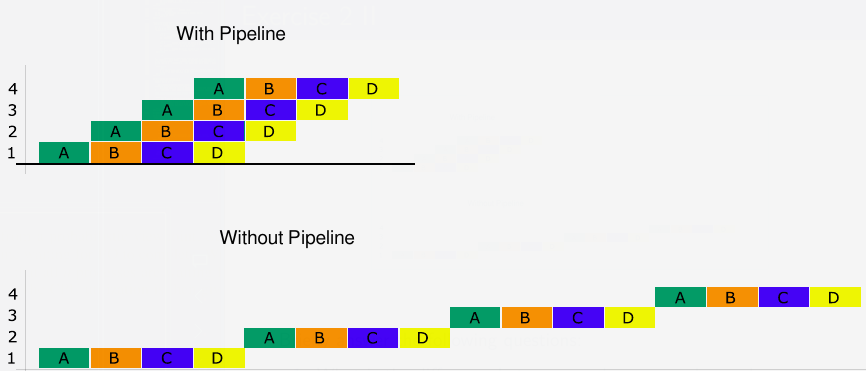
\includegraphics[keepaspectratio, width=0.8\textwidth, height=0.8\textheight-2\baselineskip-2\baselineskip]{img/010_Befehlspipeline.png} \\
    \end{figure}
    \framebreak
    
    Briefly answer the following questions:
	\begin{enumerate}
		\item What is the difference between synchronous and asynchronous interrupts?
		\alert{
		\begin{itemize}
		 \item Synchronous Interrupts: Issued by the CPU itself; exception, traps, faults e.g. page fault, syscalls
		 \item Asynchronous Interrupts: Issued by other hardware components; e.g. when network card receives a package, when DMA finished
		\end{itemize}
		}
		
	    \item What is an Advanced Programmable Interrupt Controller (APIC)?
        
	    \alert{Controller in between CPU and other HW \\
                Receives interrupts, converts to vector number, writes this to register \& raise on INTR or NMI pin, masks interrupts, distributes to local APICs}
        \begin{figure}
            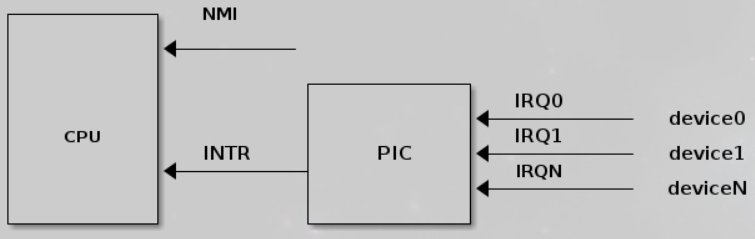
\includegraphics[keepaspectratio, width=0.8\textwidth, height=0.5\textheight-2\baselineskip-2\baselineskip]{img/010_pic.png} \\
        \end{figure}
        \begin{figure}
            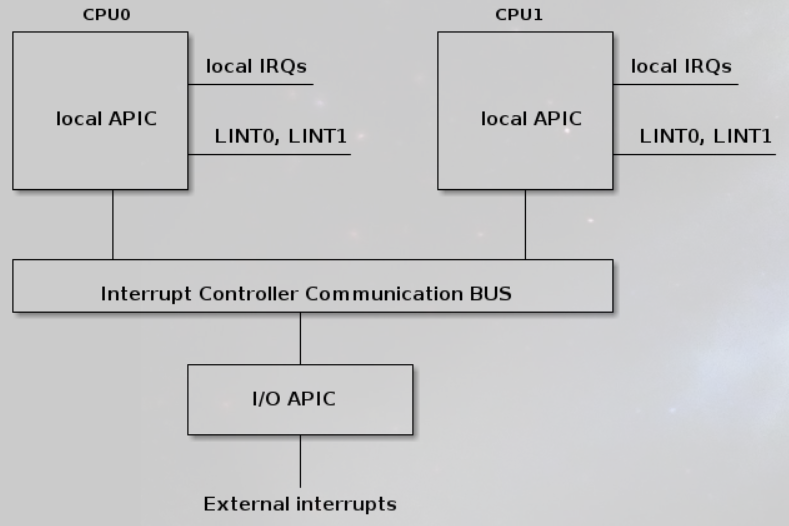
\includegraphics[keepaspectratio, width=0.8\textwidth, height=0.73\textheight-2\baselineskip-2\baselineskip]{img/010_apic.png} \\
        \end{figure}
	    
	    \item What is the Interrupt Descriptor Table? \\
	    \alert{Maps each interrupt to an interrupt handler('s address)}
	    
    	\item What is an Interrupt Handler? \\
    	\alert{A program that is called if a specific interrupt arrives. \\
    	E.g. device driver, entry point for syscalls, page fault handling, $\dots$}
    	
    	\item Which information is contained in the Extended Flags (EFFLAGS), Code Segment (CS) and EIP (Extended Instruction Pointer) registers?
    	\alert{\begin{itemize}
    	        \item EFLAGS: Status \& system flags, like carry, parity, trap, interrupts en-/disabled, privileges, overflow, $\dots$
    	        \item CS: Code Segment pointer; points to start of current process' code
    	        \item EIP: offset from CS to current instruction
    	       \end{itemize}
        }
        \framebreak
        \item How does one register an interrupt handler?
	    \alert{
	    \inputminted[autogobble, fontsize=\scriptsize]{C}{code/request_irq.c}
	    }
	    \framebreak
    	\item What is meant by ``upper half'' and ``bottom half''? What is the reason for the ``bottom half''?
    	\alert{
    	\begin{itemize}
    	 \item Upper half: Interrupts disabled. Acknowledge the IRQ, execute the handler, call end of interrupt
    	 \item Bottom half: Interrupts enabled. Handler usually queues work. Execution of this work is bottom half.
    	\end{itemize}
    	}
	\end{enumerate}
\end{frame}

\begin{frame}[allowframebreaks]{Exercise 5}
   Consider the following two-dimensional array:
    \inputminted{c}{code/array.c}
	Write a \mintinline{bash}{C} program with the functions described below.
	The output of the program should consist of three lines.
	\begin{enumerate}
		\item%
			\label{crowsdbl}%
			Write a \mintinline{bash}{C} function that receives the array as parameter and outputs it line by line:\\
			\mintinline{bash}{1 2 3 4 5 6 7 8 9 $\ldots$ 24 25 26 27 28 29 30}\\
			Use a double nested \mintinline{c}{for} loop for this.
		\item%
			\label{ccolsdbl}%
			Write a \mintinline{bash}{C} function that gets the array as parameter and outputs it column by column:\\
			\mintinline{bash}{1 7 13 19 25 2 8 $\ldots$ 29 6 12 18 24 30 }\\
			Use a double nested \mintinline{c}{for} loop for this.
		\item%
			Write a \mintinline{bash}{C} function that receives the array as parameter and outputs it line by line.\\
			Use a single, non-nested \mintinline{c}{for} loop for this.
	\end{enumerate}
    \alert{Show code}
	\begin{enumerate}
		\item[4.]%
			Let $A \in \mathbb{R}^{N \times M}$ be a matrix and let $A^T$ denote the transposed matrix.
			Is the row-major memory layout of $A$ the same as the column-major memory layout of~$A^T$?
			Rationalize your answer, e.g. with a diagram.\\
        \begin{figure}
            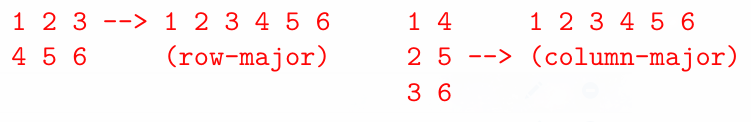
\includegraphics[keepaspectratio, width=0.8\textwidth, height=0.73\textheight-2\baselineskip-2\baselineskip]{img/060_row_col_major.png} \\
        \end{figure}
	\end{enumerate}
\end{frame}

\begin{frame}[allowframebreaks]{Exercise 6}
    Inform yourself about stackless threads.
	A possible starting point is	
	\begin{enumerate}
		\item What advantage do stackless threads offer over conventional threads?\\
		\alert{Need less memory.}
		\item What is the disadvantage of stackless threads compared to conventional threads? \\
		\alert{local variables are not preserved between thread switches $\Rightarrow$ need to use static or global vars}
		\item Do stackless threads use pre-emptive or cooperative scheduling? \\
		\alert{Cooperative}
	\end{enumerate}
\end{frame}
    
\section{Exercise sheet 3}
\frame{\sectionpage}
\begin{frame}[allowframebreaks]{}
 \begin{figure}
          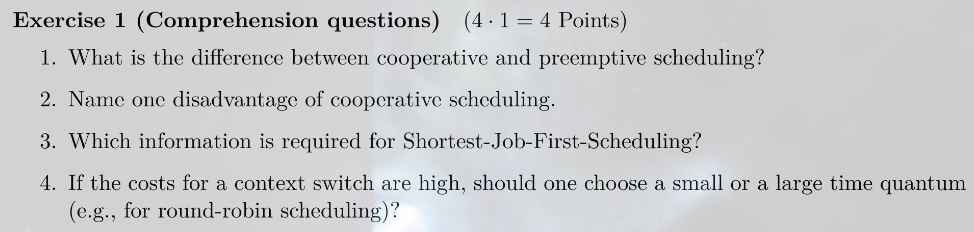
\includegraphics[keepaspectratio, width=\textwidth, height=\textheight-2\baselineskip-2\baselineskip]{img/100_ex3.png} \\
        \end{figure}
        \begin{itemize}
         \item \mintinline{c}{yield} vs. forced switch
         \item What if not yielded?
         \item How to know what's the shortest?
         \item low quantum means many switches
        \end{itemize}
        \framebreak
        
  \begin{figure}
          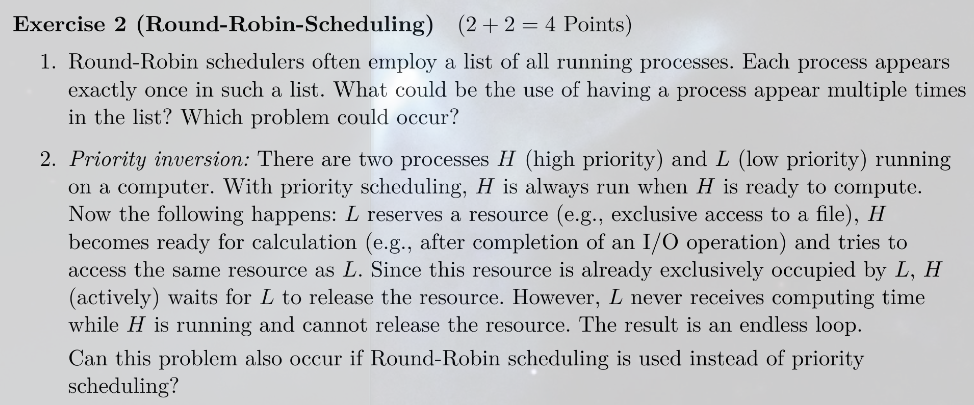
\includegraphics[keepaspectratio, width=\textwidth, height=\textheight-2\baselineskip-2\baselineskip]{img/101_ex3.png} \\
        \end{figure}
        \begin{itemize}
         \item Multiple occurrences means multiple time quanta per round. What if it blocks?
         \item Round Robin is preemptive no matter the priority
        \end{itemize}
        \framebreak
        
         \begin{figure}
          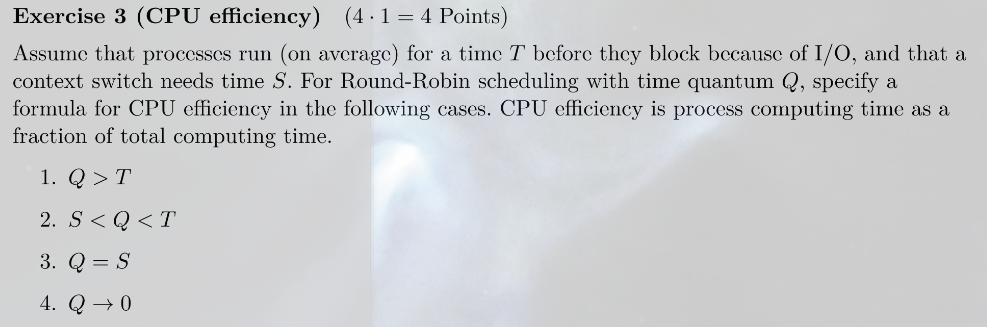
\includegraphics[keepaspectratio, width=0.8\textwidth, height=0.8\textheight-2\baselineskip-2\baselineskip]{img/102_ex3.png} \\
        \end{figure}
        \begin{itemize}
         \item Give a per process formula!
         \item Runtime = CPU time + IO time
         \item Consider how many context switches are necessary to finish the process
         \item For $Q=S$ use the previous result \& substitute
         \item What does the OS do often if the quantum is very close to zero?
        \end{itemize}
        \framebreak 
        
        \begin{minipage}{0.49\textwidth}
         \begin{figure}
          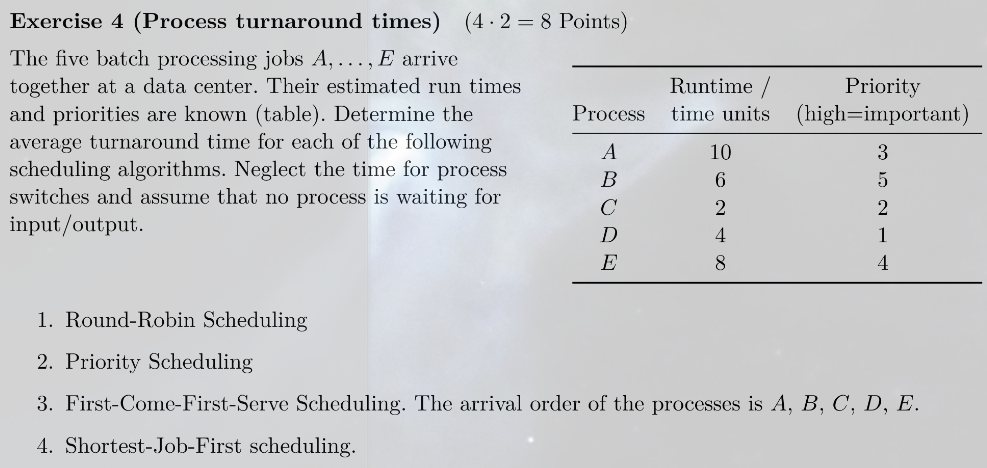
\includegraphics[keepaspectratio, width=\textwidth, height=\textheight]{img/103_ex3.png} \\
        \end{figure}
        Draw a diagram similar to the one on the left side. \\
        Popular exam exercise!
        \end{minipage} \begin{minipage}{0.49\textwidth}
        \begin{figure}
          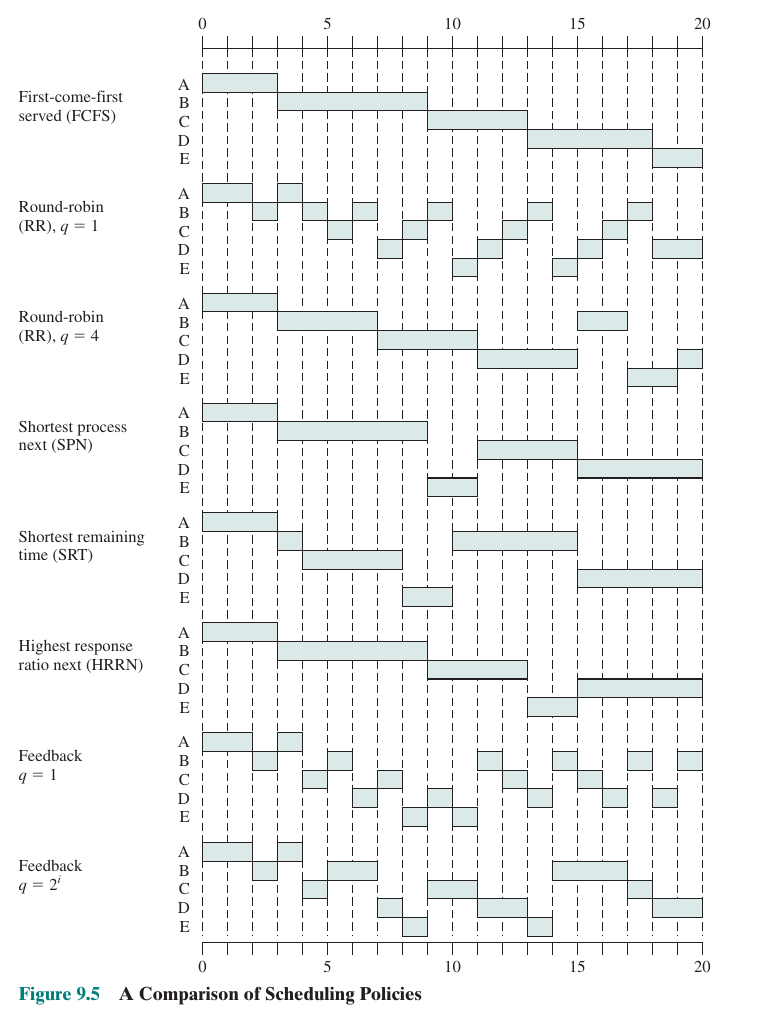
\includegraphics[keepaspectratio, width=\textwidth, height=\textheight]{img/103_sched.png} \\
        \end{figure}
        \end{minipage}
        \framebreak 
        
        \begin{figure}
          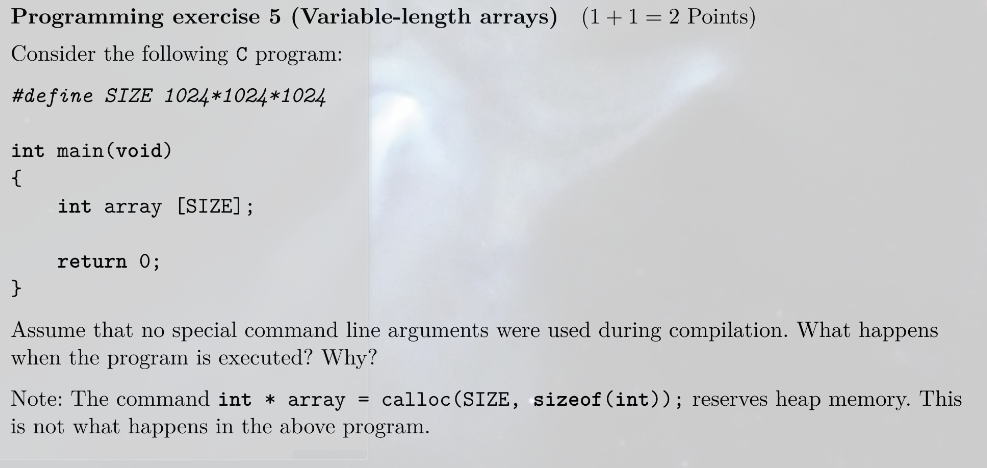
\includegraphics[keepaspectratio, width=0.8\textwidth, height=0.8\textheight-2\baselineskip-2\baselineskip]{img/104_ex3.png} \\
        \end{figure}
        Use the sanitizers! Both address and undefined!
        \framebreak 
        
        \begin{figure}
          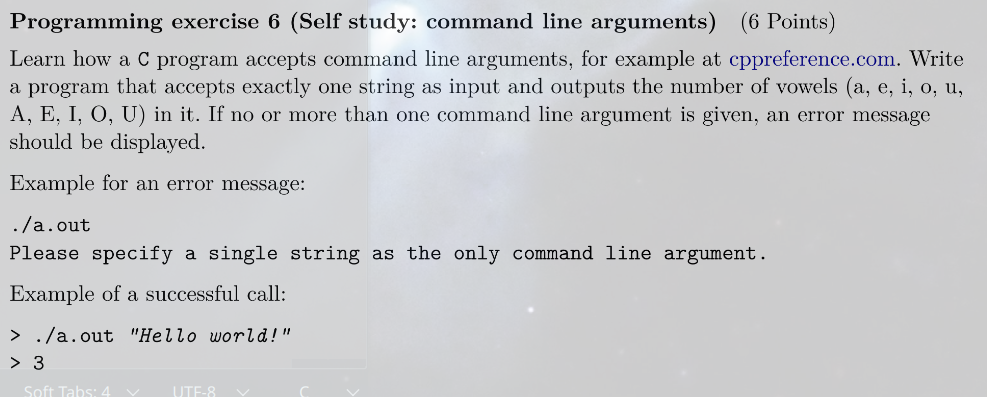
\includegraphics[keepaspectratio, width=0.8\textwidth, height=0.8\textheight-2\baselineskip-2\baselineskip]{img/105_ex3.png} \\
        \end{figure}
        Check the C programming slides or \href{https://en.cppreference.com/w/c}{the C reference}.
        \framebreak 
        
        \begin{figure}
          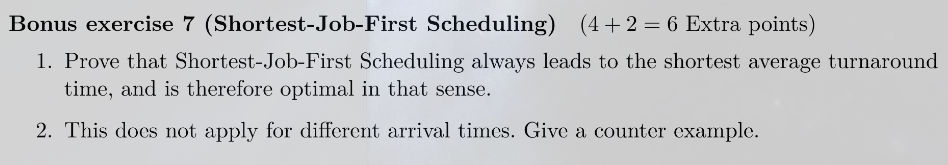
\includegraphics[keepaspectratio, width=0.8\textwidth, height=0.8\textheight-2\baselineskip-2\baselineskip]{img/106_ex3.png} \\
        \end{figure}
        Check the Tanenbaum book p. 208/209. \\
        Adapt the proof in the book to be more general.
\end{frame}

\section{References}
    \begin{frame}[allowframebreaks]
      \frametitle{References}
      \begin{tiny}
      \nocite{*}
      \printbibliography
      \end{tiny}
    \end{frame}


\end{document}
 
